
\documentclass[11pt, a4paper]{book}
\usepackage[french]{babel}
\usepackage[utf8]{inputenc}
\usepackage{answers}

\usepackage{hyperref}
\usepackage{multicol}

\usepackage[table,xcdraw]{xcolor}
\usepackage{listings}
\definecolor{ForestGreen}{RGB}{34,139,34}


\usepackage{enumitem}

\AtBeginDocument{\def\labelitemi{$\bullet$}}


\newcommand{\py}{\lstinline{Python} }


\definecolor{backcolour}{rgb}{0.95,0.95,0.92}

\lstset{%
	language         = Python,
	backgroundcolor  = \color{backcolour},
	basicstyle       = \ttfamily, % \upshape\ttfamily,
	keywordstyle     = \bfseries\color{blue}, %\bfseries,
	stringstyle      = \color{magenta},
	commentstyle     = \color{ForestGreen},
	alsoletter = > ,
	morekeywords = {>>>,as,assert,False,None, nonlocal,True, with,yield , <<, >>, :},
	showstringspaces = false,
	numbers=left,
	stepnumber=1,
	literate={à}{{\`{a}}}1 {é}{{\'e}}1 {è}{{\`{e}}}1 {ê}{{\^{e}}}1 {Ê}{{\^{E}}}1 {î}{{\^i}}1 {ô}{{\^{o}}}1 {ç}{{\c{c}}}1 {Ç}{{\c{C}}}1
}

\newcommand{\itemb}[1]{\item \textbf{#1}}

\usepackage{fancyhdr}  %package pour en-tetes et pied de pages
\usepackage{sectsty} % Permet de faire des modifications de police dans diverses sections des "headings" (cf. modif presentation de la page)
\pagestyle{fancy}       %Style pour en-tetes et pieds de pages
\fancyhead[CO,CE]{\sc Série 1\hspace{0.5mm}}
\fancyhead[RO,LE]{Collège Sismondi}  % LaTeX/TEX define \strut to be an invisible box of width zero that extends just enough above and below the baseline. Cela permet d'augementer légèrement la taille en bas de la box de manière à ce qu'elle soit collée à la ligne.
\fancyhead[LO,RE]{\small\ \textsl{1\textsuperscript{ère} année - DO Informatique}}
\fancyfoot[RO,LE]{2021 - 2022}
\fancyfoot[LO,RE]{\small }
\fancyfoot[CO,CE]{\thepage}

\fancyhfoffset[l]{1.2cm} % le "l" en paramètre permet d'indiquer qu'on ne veut modifier que la marge à gauche.
\renewcommand{\headrule}{{%
		\hrule \headwidth \headrulewidth \vskip-\headrulewidth}}
\renewcommand\footrulewidth{\headrulewidth}
\renewcommand{\footrule}{{%
		\vskip-\footruleskip\vskip-\footrulewidth
		\hrule \headwidth \footrulewidth\vskip\footruleskip}}

\usepackage{tikz}
%-------------------------------------------------------------------------------
%---- Eclairage : en encadré sur fond jaune avec symbôle "ampoule" à gauche ----
%-------------------------------------------------------------------------------
\definecolor{coleclairage}{RGB}{255 , 221 , 156}
\definecolor{contoureclairage}{RGB}{255 , 192 , 0}
\newenvironment{eclairage}
{
	\begin{center}%
		\begin{tikzpicture}%
			\node[rectangle, draw=contoureclairage, top color=coleclairage!50, bottom color=coleclairage!140, rounded corners=5pt, inner xsep=5pt, inner ysep=6pt, outer ysep=10pt]\bgroup                     
			\begin{minipage}{0.98\linewidth}
				\begin{minipage}{0.08\linewidth}\centerline{
\includegraphics[scale=1]{Symbole_eclairage.png}}\end{minipage}
				\begin{minipage}{0.89\linewidth}\itshape\footnotesize
				}
				{                		
				\end{minipage}
			\end{minipage}\egroup;%
		\end{tikzpicture}%
	\end{center}%
}

%-------------------------------------------------------------------------------
%---- apprendre : en encadré sur fond jaune avec symbôle "ampoule" à gauche ----
%-------------------------------------------------------------------------------
\definecolor{colapprendre}{RGB}{50,205,50}
\definecolor{contourapprendre}{RGB}{34,139,34}
\newenvironment{apprendre}
{
	\begin{center}%
		\begin{tikzpicture}%
			\node[rectangle, draw=contourapprendre, top color=colapprendre!10, bottom color=colapprendre!50, rounded corners=5pt, inner xsep=5pt, inner ysep=6pt, outer ysep=10pt]\bgroup                     
			\begin{minipage}{0.98\linewidth}
				\begin{minipage}{0.08\linewidth}\centerline{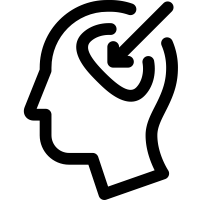
\includegraphics[width=30px]{Symbole_learn.png}}\end{minipage}
				\begin{minipage}{0.89\linewidth}\itshape\footnotesize
				}
				{                		
				\end{minipage}
			\end{minipage}\egroup;%
		\end{tikzpicture}%
	\end{center}%
}

\definecolor{colimportant}{RGB}{247 , 189 , 164}
\definecolor{contourimportant}{RGB}{237 , 125 , 49}
\newenvironment{important}
{
	\begin{center}%
		\begin{tikzpicture}%
			\node[rectangle, draw=contourimportant, top color=colimportant!50, bottom color=colimportant!140, rounded corners=5pt, inner xsep=5pt, inner ysep=6pt, outer ysep=10pt]\bgroup                     
			\begin{minipage}{0.08\linewidth}\centerline{
\includegraphics[scale=0.8]{Symbole_attention.png}}\end{minipage}
			\begin{minipage}{0.89\linewidth}
			}
			{                		
			\end{minipage}\egroup;
		\end{tikzpicture}%
	\end{center}%
}

%-----------------------------------------------------------------
%---- Modification présentation de la page: marges de la page ----
%-----------------------------------------------------------------
%\addtolength{\hoffset}{-1in}              % 1
%\addtolength{\voffset}{-1in}              % 2
\addtolength{\oddsidemargin}{-0.1 in} % 3
\addtolength{\evensidemargin}{-1in} % 3
\addtolength{\topmargin}{-1in}       % 4
\addtolength{\headheight}{6pt}       % 5
%\addtolength{\headsep}{-0.2cm}           % 6
\setlength{\textheight}{26cm}    % 7
\setlength{\textwidth}{16.5cm}      % 8
\addtolength{\marginparsep}{0pt}      % 9
\setlength{\marginparwidth}{0pt}   % 10
\addtolength{\footskip}{-1mm}           %11

\setlength{\parindent}{0em}% pas d'indentation


% Customiser le nom des sections
\usepackage{titlesec}
\titleformat{\section}[hang]{\Large \bfseries}{Série \thesection:\ }{0pt}{}

\renewcommand{\familydefault}{\sfdefault} % pour avoir des polices san serif

\newtheorem{Exc}{Exercice}
\Newassociation{correction}{Soln}{mycor}
\renewcommand{\Solnlabel}[1]{\bfseries Ex #1 }
\def\exo#1{%
	\futurelet\testchar\MaybeOptArgmyexoo}
\def\MaybeOptArgmyexoo{
	\ifx[\testchar \let\next\OptArgmyexoo
	\else \let\next\NoOptArgmyexoo \fi \next}
\def\OptArgmyexoo[#1]{%
	\begin{Exc}[#1]\normalfont}
	\def\NoOptArgmyexoo{%
		\begin{Exc}\normalfont}
		\newcommand{\finexo}{\end{Exc} \vspace{3mm}}
	\newcommand{\flag}[1]{}
	\newcommand{\entete}[1]

\newcommand{\getexocompteur}{{\the\numexpr \arabic{Exc}  \relax}}	
	
\newcommand{\eexo}{\vspace{5mm}} % espace pour séparer les exercices
\pgfplotsset{compat=1.17}
\begin{document}

\setcounter{chapter}{4}

\chapter{Ordinateurs}

\section{Qu’est-ce qu’un ordinateur (computer) ?}

\begin{defi}
	Un ordinateur est une machine électronique capable de traiter (calculer, stocker) des données de manière automatisée et optimisée à l'aide de logiciels, ainsi que de les partager au travers d'un réseau et de périphériques. 
\end{defi}

\begin{center}
\begin{figure}[ht!]
	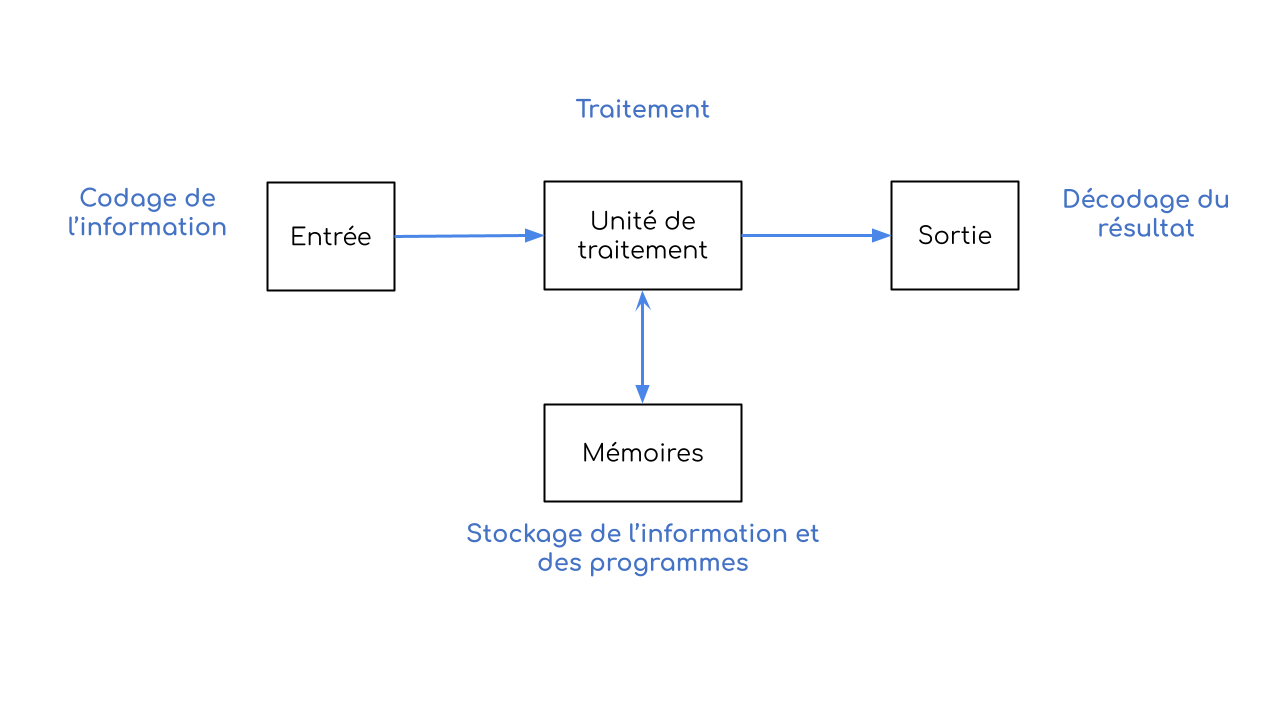
\includegraphics[scale=.4]{images/shema_ordinateur.png}
	\caption{Schéma fonctionnel de l'ordinateur}
\end{figure}
\end{center}
	
	On parle souvent de PC (Personnal Computer) ou ordinateur personnel. C'est tout simplement un ordinateur qui répond aux besoins des utilisateurs (humains).

\begin{center}
\begin{figure}[h]
	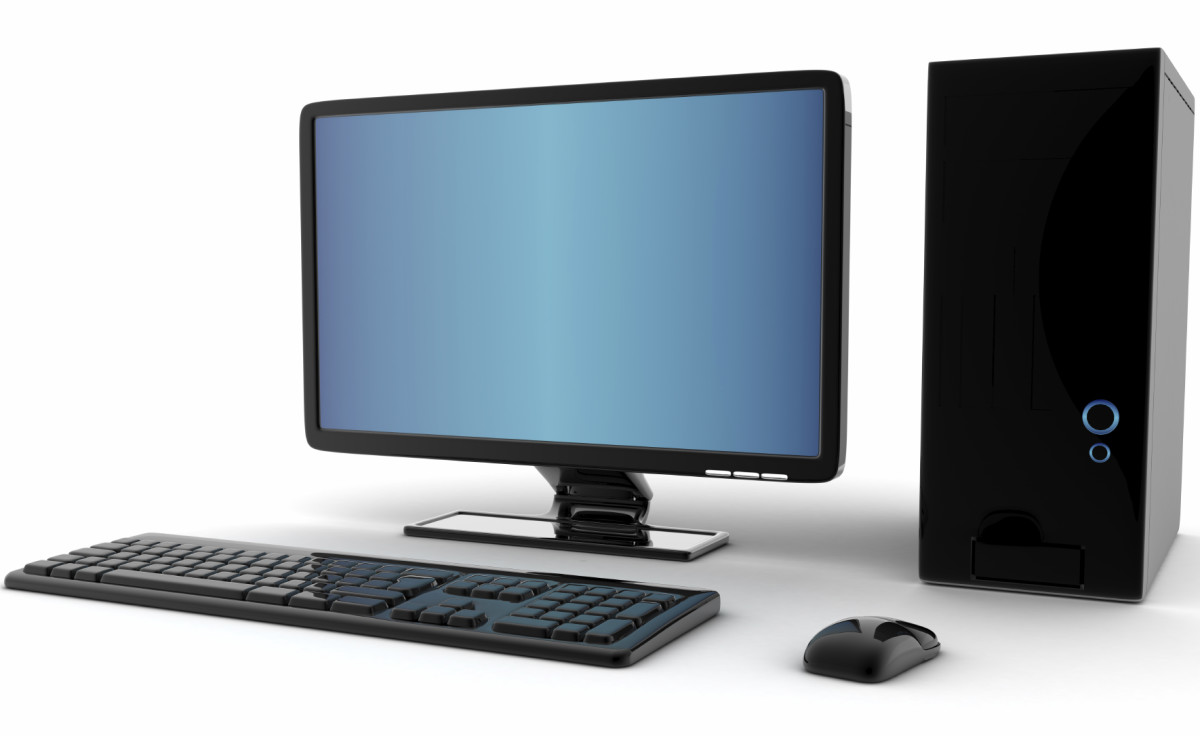
\includegraphics[scale=.3]{images/ordinateur}
	\caption{Exemple d'ordinateur personnel}
\end{figure}
\end{center}
	
	
	
Il existe des ordinateurs plus puissants qui sont spécialement conçus pour fournir des informations et des logiciels à d'autres ordinateurs reliés via un réseau. On les appelle des {\bf serveurs}. Ces derniers sont capables de traiter des charges de travail plus importantes et d'exécuter davantage d'applications.


\begin{figure}[h]
	\centering
	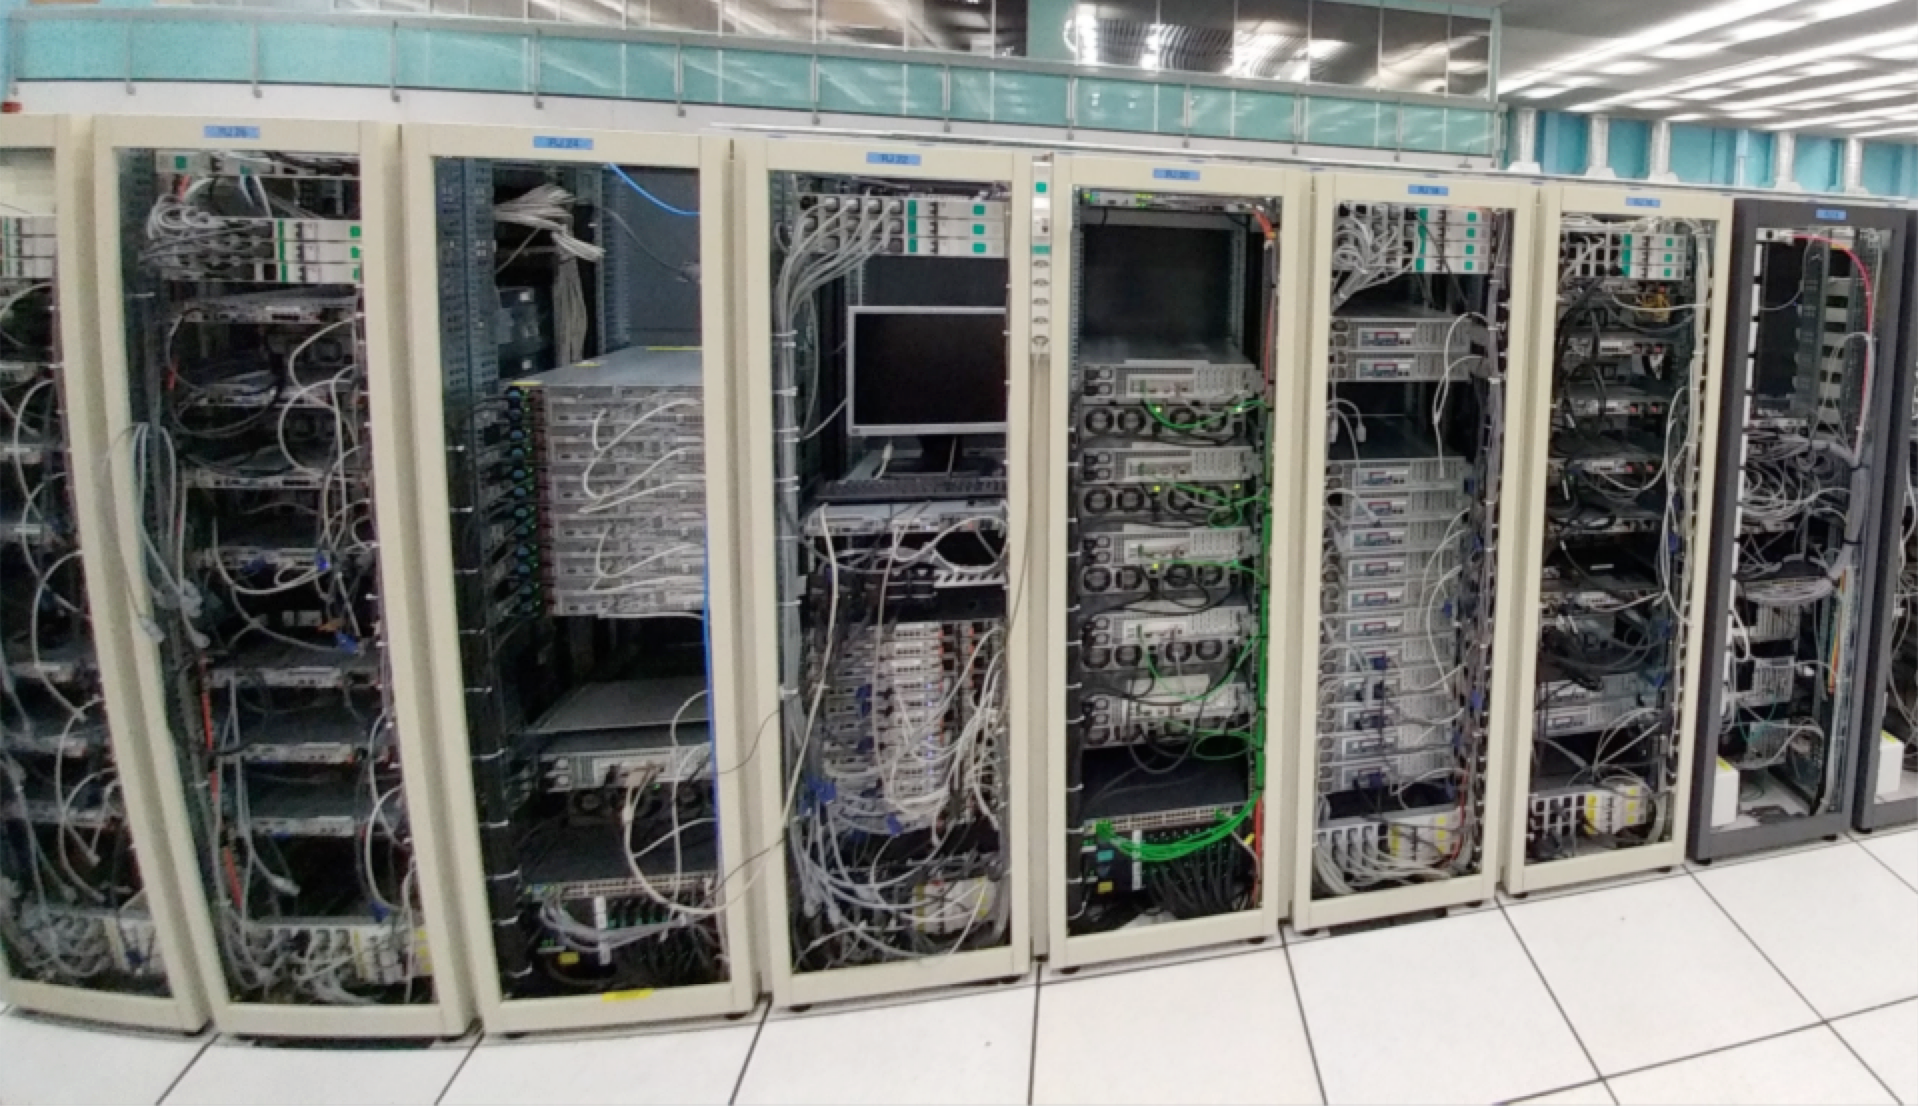
\includegraphics[scale=.4]{images/serveur}
	\caption{Salle de serveurs du CERN}
	\label{serveur}
\end{figure}


Les ordinateurs les plus puissants au monde sont appelés supercalculateur. Ils contiennent des centaines, voire des milliers de processeurs. Ils sont souvent utilisés dans la recherche médicale, les applications scientifiques (cf Figure \ref{serveur}), le domaine de la finance, la météorologie et à des fins militaires.


\section{L'intérieur d'un ordinateur}

\subsection{Les composants}

Pour fonctionner, l’ordinateur est constitué de composants électroniques comme la mémoire (4) ou le processeur (2). Ces composants sont regroupés sur une carte mère (1) qui est le circuit imprimé \footnote{Le circuit imprimé est un support, en général une plaque, permettant de maintenir et de relier électriquement un ensemble de composants électroniques entre eux.} principal. Elle permet de prendre en charge la mémoire vive (4), la lecture du disque dur (7) et l'utilisation du processeur. Cette carte mère est fixée à l'unité centrale également nommée : la tour, le boîtier, desktop, etc.

\begin{center}
\begin{figure}[h]
	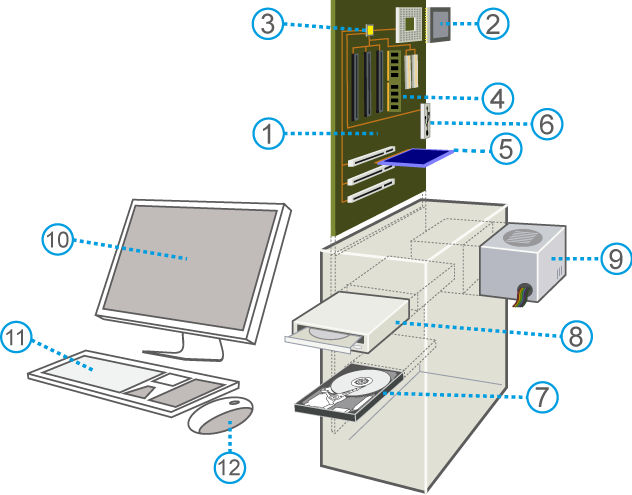
\includegraphics[scale=.6]{images/composants}
	\caption{L'ordinateur, l'unité centrale et sa composition}
	\label{composants}
\end{figure}
\end{center}

Les principaux composants constituant un ordinateur sont :
\begin{itemize}%[label=\textbullet]
    \item Le {\bf processeur} (CPU, Central Processing Unit) (2) : il gère tous les calculs pour permettre à l'ordinateur de fonctionner. Il va exécuter une suite l'instruction cadencée par une horloge (la fréquence du processeur). Il permet donc d'exécuter différents programmes. Il va s'appuyer sur la mémoire vive pour stocker ses calculs.
      
    \item  La {\bf mémoire vive} (Random Access Memory) (4) : c'est une mémoire très rapide où se trouvent les informations traitées par le processeur. Lorsque l'ordinateur est éteint, les informations contenues en mémoire vive ne sont plus maintenues, on perd l'information.

    \item La {\bf mémoire permanente} : est une mémoire moins rapide que la mémoire vive, mais de plus grande capacité utilisée pour sauvegarder des données. Le disque dur (hard drive) (7) est un exemple de mémoire permanente.
      
    \item  Le {\bf lecteur/graveur CD/DVD/Blu-ray } (8) : il lit l'ensemble des CD, DVD et Blu-ray, que ce soit de la musique, des logiciels, des jeux, des films, etc.
      
    \item L'{\bf alimentation} (9) : branchée sur le réseau électrique 220 [V], elle alimente tous les composants électroniques.
      
    \item La {\bf carte graphique} (graphic card) (5) : elle transmet les images qu'elle possède en mémoire sur les écrans. Elle permet donc d'afficher à l'écran des images, du texte, des vidéos, etc. en allumant des points lumineux (pixels). À noter que certains processeurs comportent une unité graphique rendant obsolète l'ajout d'une carte graphique sur un ordinateur, typiquement pour un usage de type bureautique.
\end{itemize}

\begin{remarque}
Dans un smartphone, c'est le {\bf SoC, (system on a chip)} qui rassemble quasiment tous ces composants: CPU, GPU (processeur de la carte graphique), modem (connexion réseau), mémoire RAM... Dans une petite puce (M1 ou A11 par exemple chez apple ou Exynos chez Samsung) se retrouve concentrée la puissance d'un ordinateur d'il y a quelques années.
\end{remarque}

\subsection{ Caractéristiques des composants}


\subsubsection{La carte mère}

Une {\bf carte mère} se distingue principalement par la génération de processeur qu'elle peut accueillir, par le type de mémoire vive pouvant être connecté, le nombre et les différents types de connecteurs (6) (IDE, sata, PCI, etc.) qu'elle comporte  et par son jeu de composants électroniques (chipset) lui permettant de gérer l'échange de données entre les disques, la mémoire, la carte graphique et les différents périphériques externes d'entrée/sortie. La carte mère comporte également un ensemble de fonctions nommé BIOS ({\it Basic Input Output System}) ou plus récemment UEFI ({\it Unified Extensible Firmware Interface}) lui permettant, lors de sa mise sous tension, d'identifier le matériel connecté sur la carte mère.

\begin{figure}[h]
	\centering
	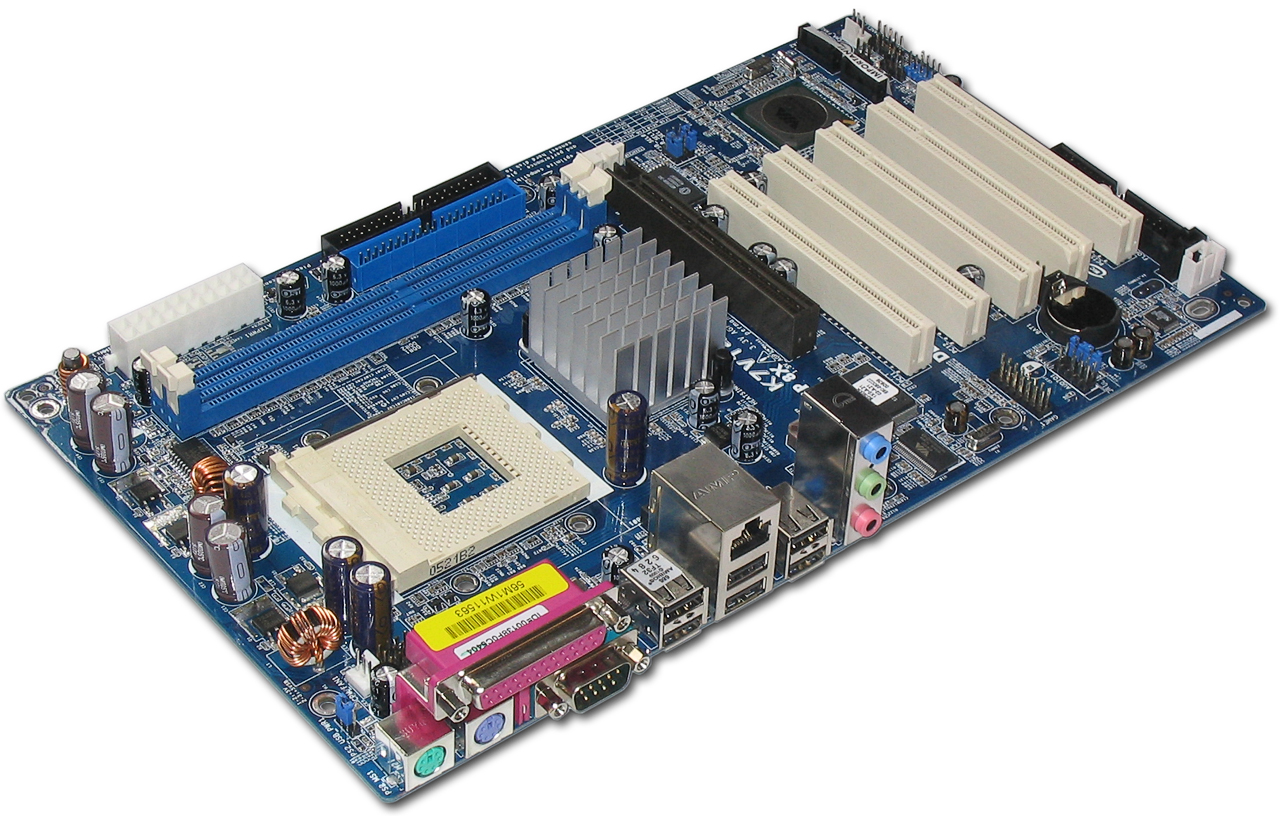
\includegraphics[scale=.4]{images/cartemere}

\end{figure}

\subsubsection{Processeur}

Un processeur se distingue principalement par sa fréquence de fonctionnement et son architecture. À l’heure actuelle, sa fréquence se traduit en gigahertz [GHz]. Concrètement, une fréquence de 2 GHz signifie que le processeur peut réaliser deux milliards d'opérations à la seconde. Parmi les entreprises réputées dans la conception de processeur, on trouve : AMD, IBM, Intel, Hewlett-Packard, Hitachi, Oracle, Motorola, Texas Instrument.

\begin{figure}[h]
	\centering
	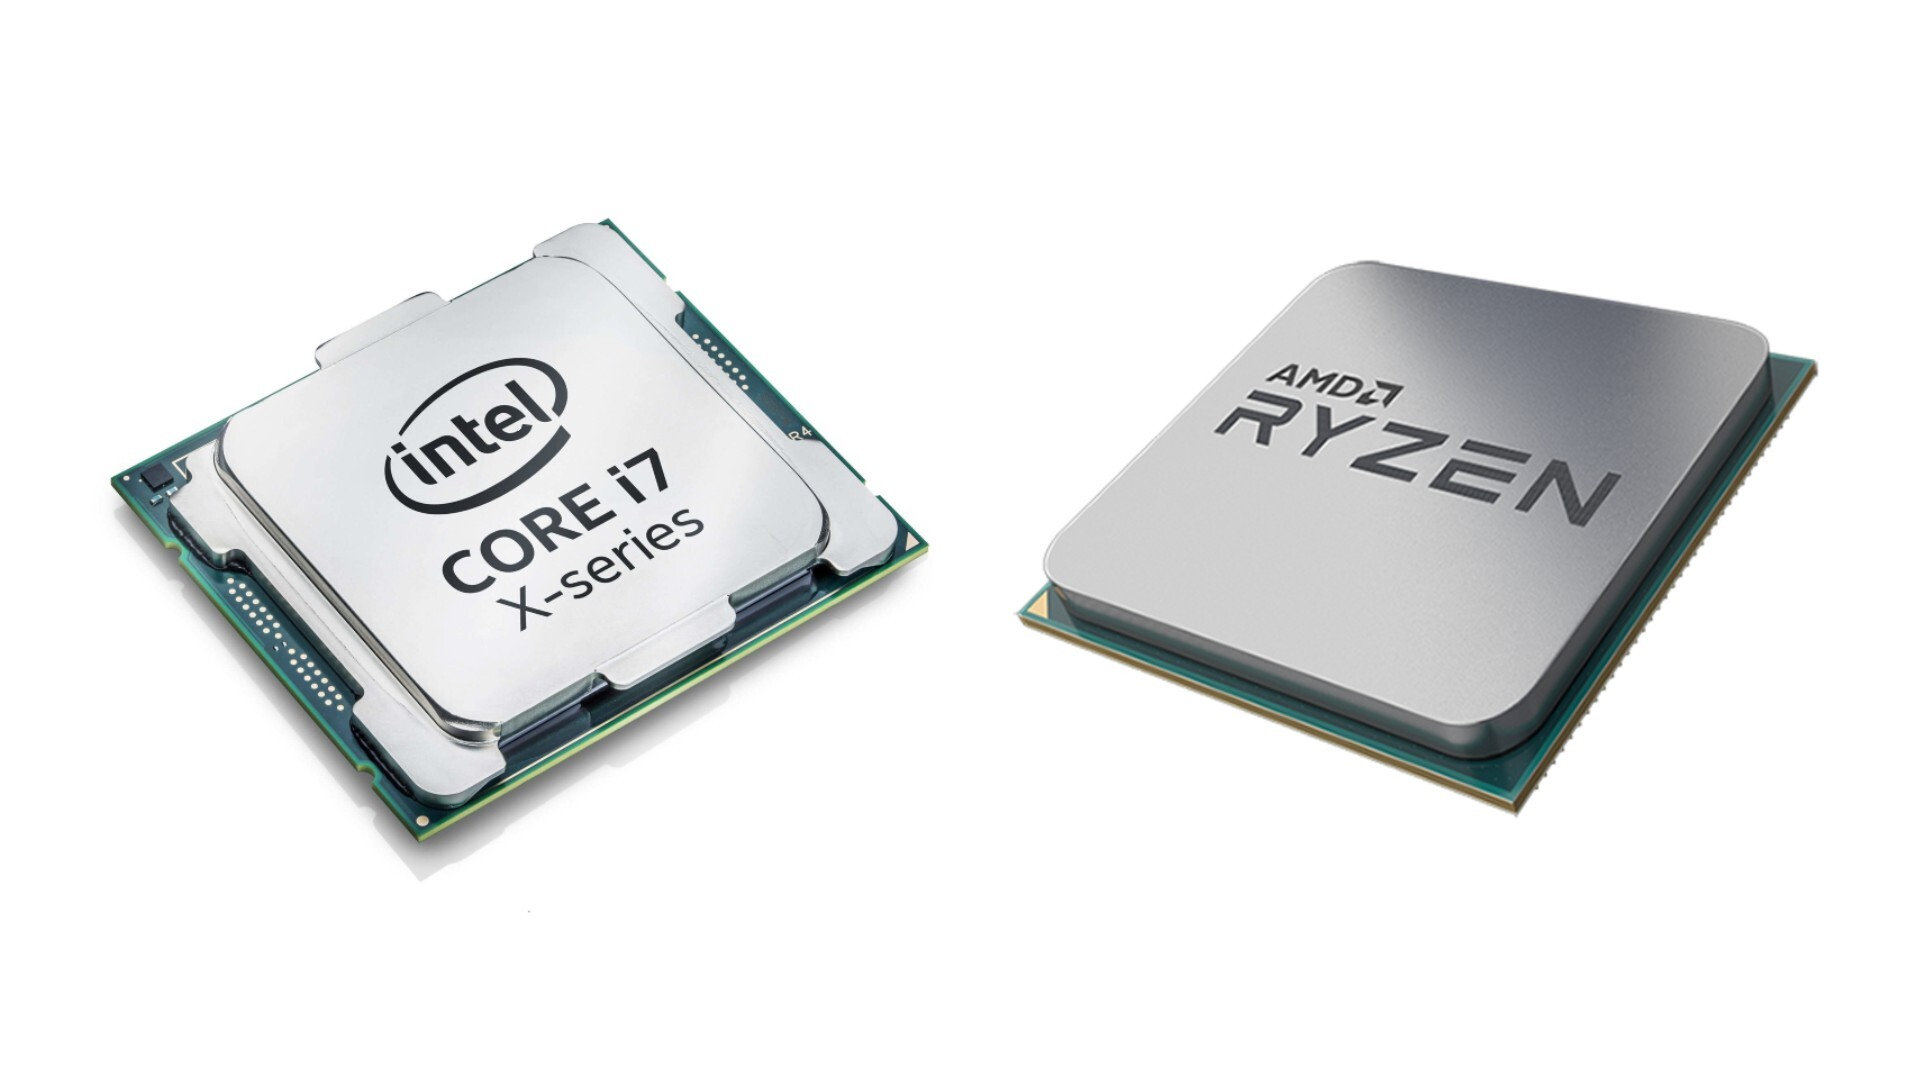
\includegraphics[scale=.15]{images/processeur}

\end{figure}


\subsubsection{Mémoire}

Qu'il s'agisse de {\bf mémoire vive} ou {\bf mémoire permanente}, la mémoire est principalement caractérisée par sa capacité de stockage et sa rapidité d'accès en lecture et en écriture. Actuellement, sa capacité est traduite en gigaoctets [Go] ou téraoctets [To]. La vitesse de lecture et d'écriture est donnée en Mo/s.

\begin{figure}[h]
	\centering
	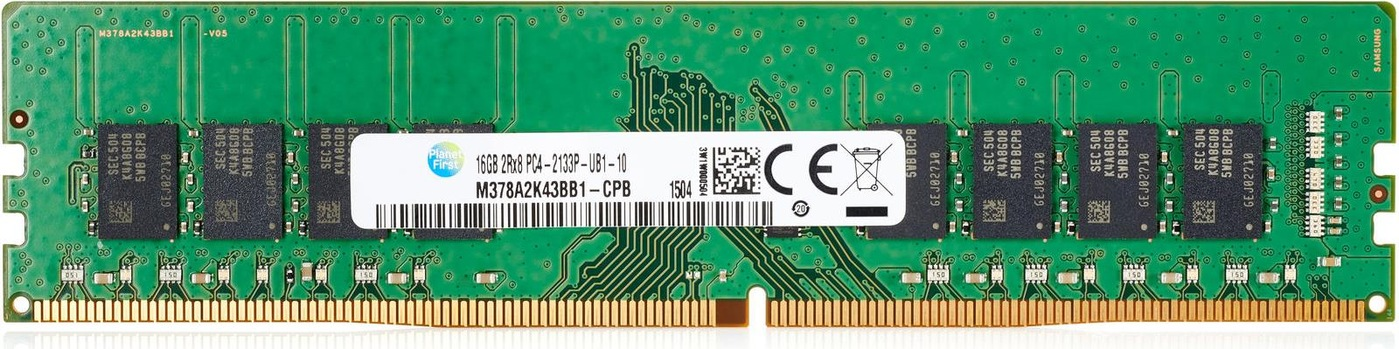
\includegraphics[scale=.3]{images/sdram}

\end{figure}





\subsubsection{L'alimentation}

L’{\bf alimentation } est caractérisée par sa puissance. La puissance de l'alimentation détermine la quantité d'électricité délivrée en watts [W]. Elle permet de fournir un courant continu nécessaire aux circuits électroniques. Les alimentations comportent une certification (label) donnant une garantie d'économie d'énergie. Ce label est accordé aux alimentations dont le rendement – rapport entre puissance fournie et consommée – est supérieur à 80 \%.

\begin{figure}[h]
	\centering
	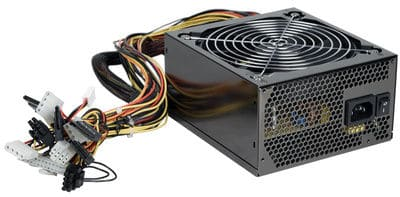
\includegraphics[scale=.5]{images/alimentation}

\end{figure}

\subsubsection{La carte graphique}

	La {\bf carte graphique} se caractérise principalement par l'architecture de son processeur graphique (GPU) et sa mémoire vive. À ce jour, Nvidia et AMD sont leaders dans la conception des processeurs graphiques. On distingue très facilement les cartes graphiques les plus puissantes par le système de refroidissement qu’elle possède.
	
	\begin{figure}[h]
	\centering
	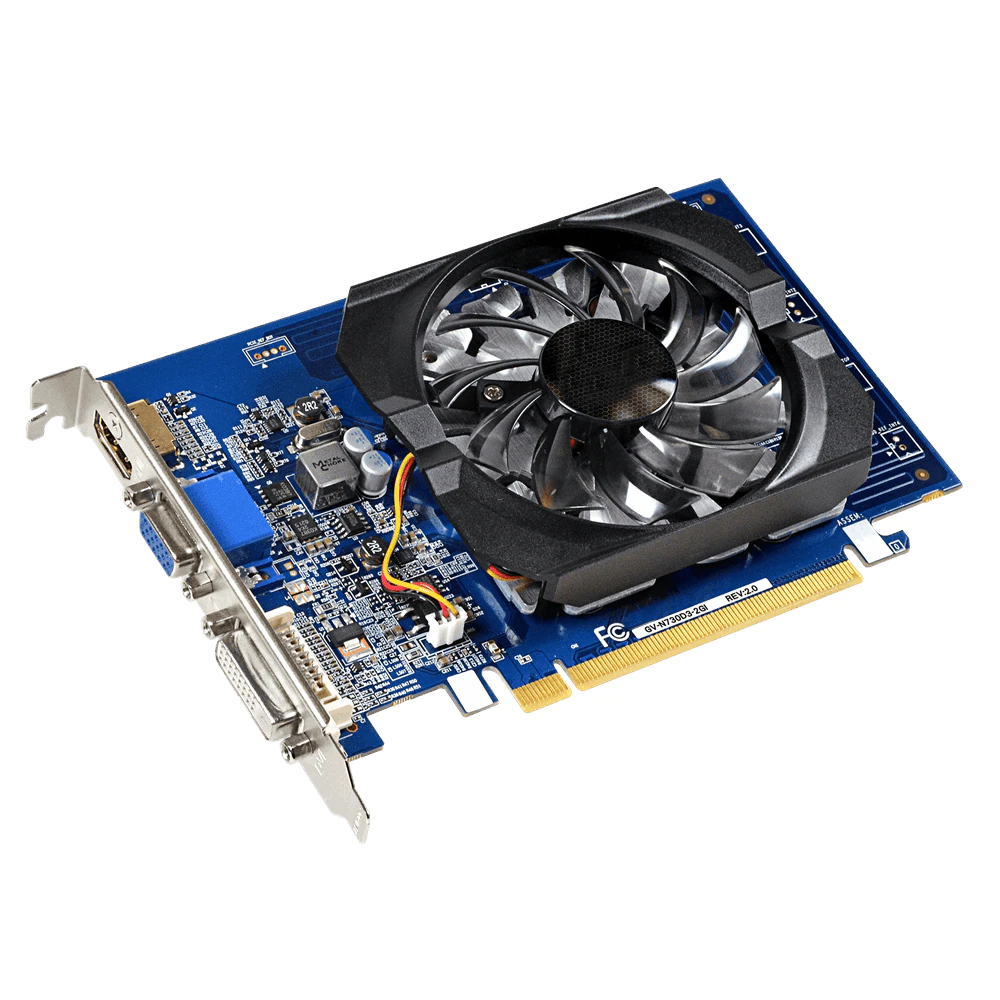
\includegraphics[scale=.2]{images/carte_graphique}

\end{figure}



\section{Périphériques externes}

\subsection{Exemples de périphériques}

Pour interagir avec l’ordinateur, des périphériques d’entrée/sortie sont nécessaires. Il en existe de toutes sortes et ces derniers sont connectés à l’ordinateur par différent type de câbles (réseau, USB, DVI, série, etc.) ou à l’aide d’une connexion sans fils (infrarouge, wifi, Bluetooth, lasers, etc).

\begin{figure}[h]
	\centering
	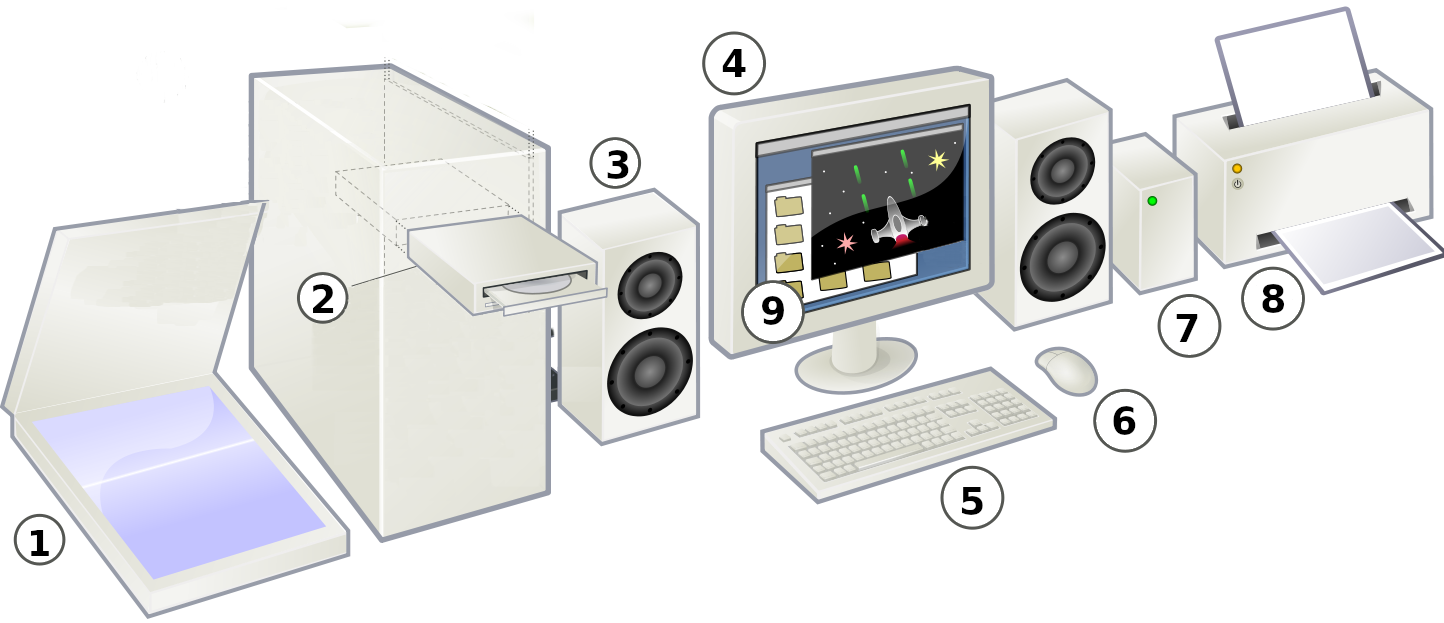
\includegraphics[scale=.3]{images/peripherique}
	\caption{Périphériques d'un ordinateur}
\end{figure}


Les différents types de périphériques externes sont :
\begin{enumerate}[1)]
    \item Le {\bf scanner} permet la numérisation de document dans une certaine résolution.
    \item Le {\bf lecteur} CD ou DVD ou Blu-ray sont des lecteurs permettant de lire un support amovible à l’aide d’un faisceau laser.
    \item Le {\bf haut-parleur} permet de diffuser du son.
    \item L’{\bf écran} permet d’afficher les informations, mais lorsqu’il est tactile, il offre la possibilité de se passer de la souris et du clavier. Il est caractérisé par sa taille et sa définition d’écran qui est le nombre de points ou pixels que peut afficher un écran. Actuellement, les définitions (nombre de points H x V) les plus courantes sur un écran pour ordinateur sont :
    	\begin{itemize}
            	\item XGA : 1024 x 768
            	\item  HD : 1280 x 768
            	\item  Full HD : 1920 x 1080
            	\item WUXGA : 1920 x 1200
            	\item  WQHD : 2560 x 1440
            	\item 8K Full Format : 8192 x 4320
           \end{itemize}
    \item le {\bf clavier}. utilisé pour écrire, mais également se déplacer rapidement dans un texte ou dans des menus, voire même effectuer une copie d’écran (screenshot).
    \item La {\bf souris} sert à déplacer le curseur sur l’écran, de choisir des applications et aussi de cliquer sur des icônes pour démarrer des logiciels. Elle permet de naviguer sur votre ordinateur, mais également de dessiner, sélectionner des textes, etc. Elle est mobile avec ou sans fil.
    \item Le {\bf disque externe} est un disque dur qui n’est pas intégré dans l’ordinateur. En fonction de sa taille, il peut être facilement déplacé. En fonction du modèle, les disques externes sont soit alimentés par un branchement USB, soit avec une alimentation sur secteur 220[V].
    \item L’{\bf imprimante} 2D permet l’impression de texte, image, graphique. Il existe plusieurs technologies d’impressions telles que laser, jet d’encre, sublimation, etc. Depuis les années 2010, l’impression 3D prend de l’ampleur avec l’arrivée de nouvelles technologies innovantes basées sur de nouveaux matériaux comme le plastique, la cire, le métal, la céramique, le verre. Il est même possible d’imprimer en 3D une forme en chocolat !
    \item L’{\bf interface graphique} ou l’{\bf environnement graphique} est un dispositif logiciel permettant le dialogue entre l’utilisateur·trice et l’ordinateur.
En fonction de son utilisation, un périphérique est considéré soit en entrée, soit en sortie, soit comme étant bidirectionnel. Le tableau suivant résume le type de périphérique.
\end{enumerate}





\subsection{Périphériques d'entrée et de sortie}

En fonction de son utilisation, un périphérique est considéré soit en entrée, soit en sortie, soit comme étant bidirectionnel. Le tableau suivant résume le type de périphérique.

Si le périphérique envoie des données à l'ordinateur, on l'appelle un {\bf périphérique d'entrée}.

Si le périphérique reçoit des données de l'ordinateur, on l'appelle un {\bf périphérique de sortie}

Un périphérique peut aussi envoyer et recevoir des données de l'ordinateur: c'est un {\bf périphérique d'entrée et de sortie}.

\section{Système d'exploitation}

Pour qu’un ordinateur soit capable de faire fonctionner un programme informatique (appelé parfois application ou logiciel), la machine doit être en mesure d’effectuer un certain nombre d’opérations préparatoires afin d’assurer les échanges entre le processeur, la mémoire, et les ressources physiques (périphériques). C'est le système d'exploitation qui s'en occupe:

\begin{defi}
	Le {\bf système d’exploitation} (noté SE ou OS, abréviation du terme anglais Operating System) est chargé d’assurer la liaison entre les ressources matérielles, l'utilisateur et les applications (traitement de texte, jeu vidéo..). 
\end{defi}	

\begin{figure}[h]
	\centering
	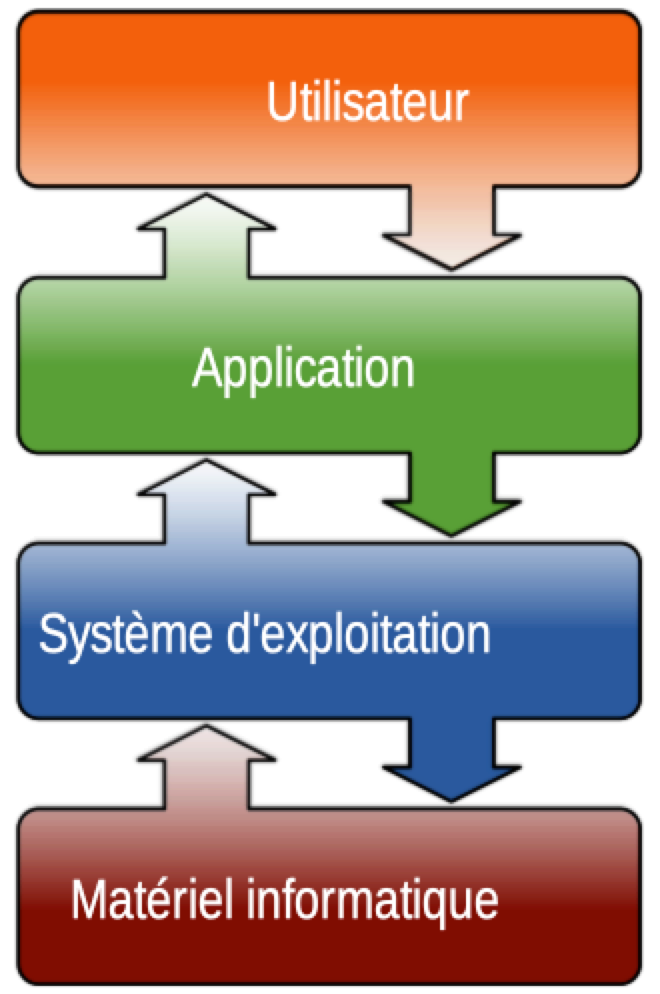
\includegraphics[scale=.3]{images/systemeexploitation}
\end{figure}
	
	Ainsi, lorsqu’un programme désire accéder à une ressource matérielle, il ne lui est pas nécessaire d’envoyer des informations spécifiques au périphérique, il lui suffit d’envoyer les informations au système d’exploitation, qui se charge de les transmettre au périphérique concerné via son pilote:
	
	\begin{defi}
		Un {\bf pilote} (ou {\bf driver} est un programme particulier qui permet la bonne liaison entre l'ordinateur et un périphérique particulier (scanner, imprimante...).
	
	\end{defi}
	
	En l’absence de pilotes, il faudrait que chaque programme reconnaisse et prenne en compte la communication avec chaque type de périphérique !
	
	Le système d’exploitation permet ainsi de « dissocier » les programmes et le matériel, afin
notamment de simplifier la gestion des ressources et offrir à l’utilisateur une interface humain – machine simplifiée afin de lui permettre de s’affranchir de la complexité de la machine physique.	
	
	
	Il existe de nombreux systèmes d’exploitation. Les plus connus à ce jour sont : Microsoft Windows, GNU/Linux, Apple Mac OS, Oracle Solaris, Google Android, etc.

\begin{figure}[h]
	\centering
	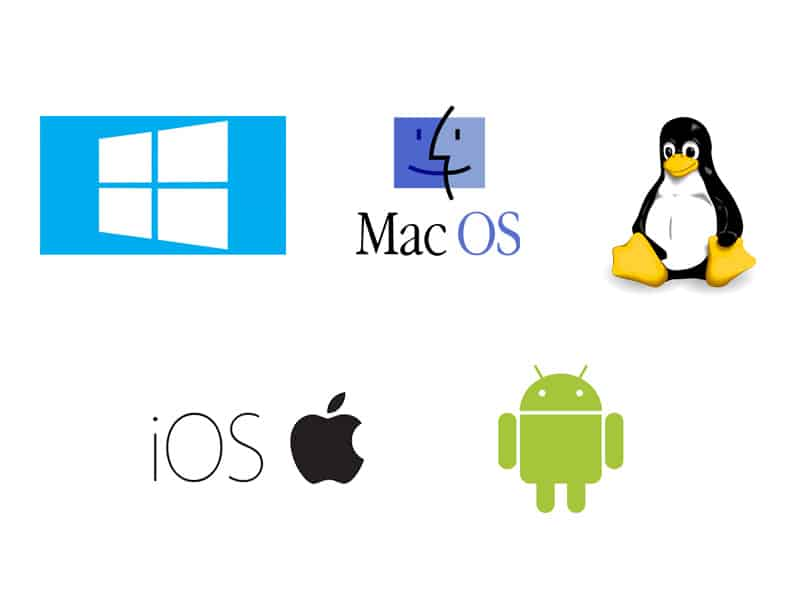
\includegraphics[scale=.3]{images/OS}
	\caption{Différents systèmes d'exploitation}
\end{figure}


\newpage

\section{Exercices}


\begin{exercice}
Relie chaque composant à son nom:

\begin{tikzpicture}
	\node (image1) at (0,0) {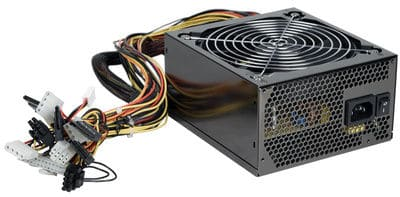
\includegraphics[width=4cm]{images/alimentation}};
	\node (image2) at (0,3) {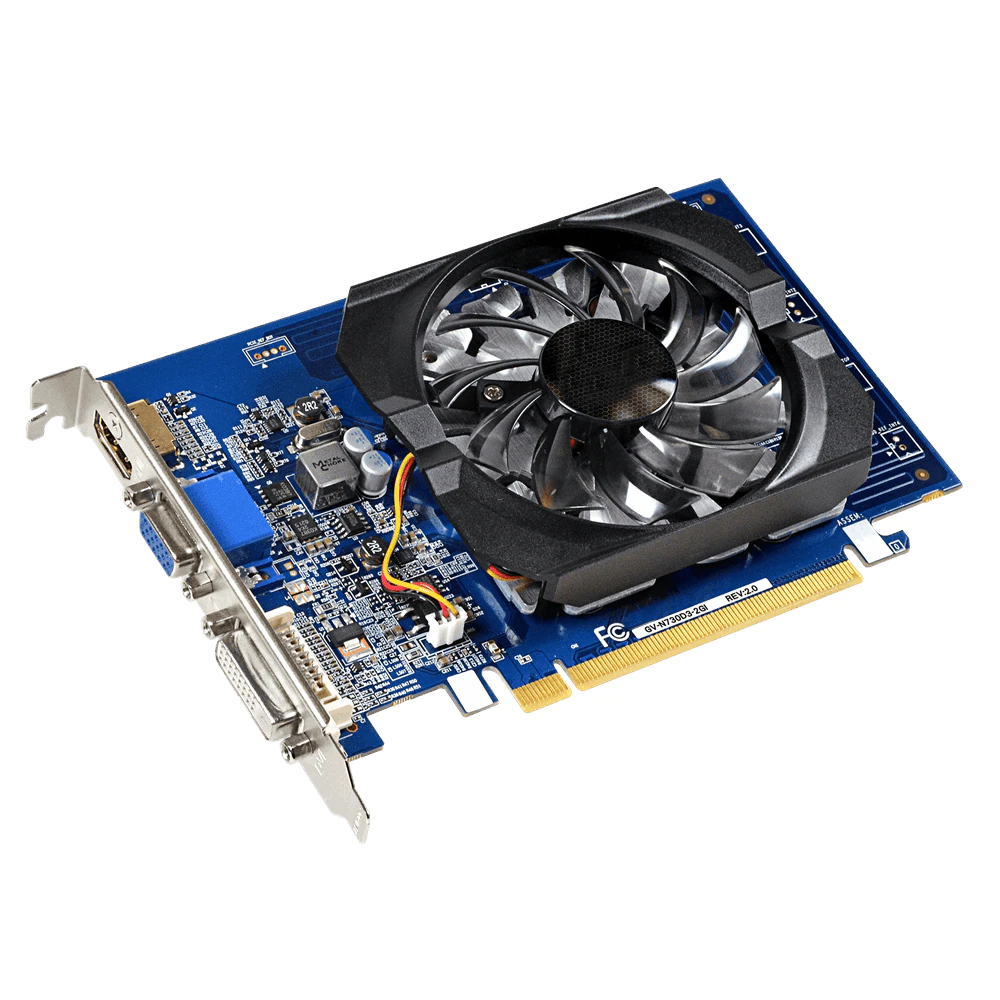
\includegraphics[width=4cm]{images/carte_graphique}};
	\node (image3) at (0,6) {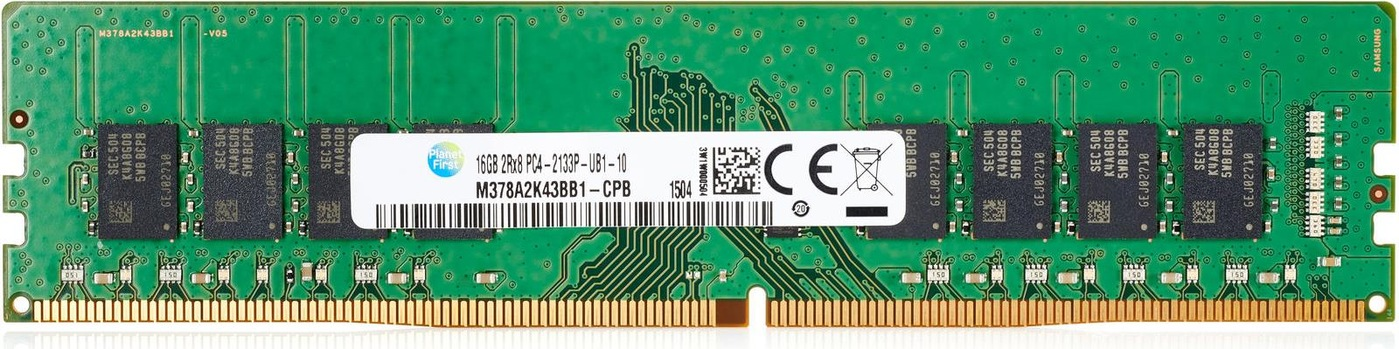
\includegraphics[width=4cm]{images/sdram}};
	\node (image4) at (0,9) {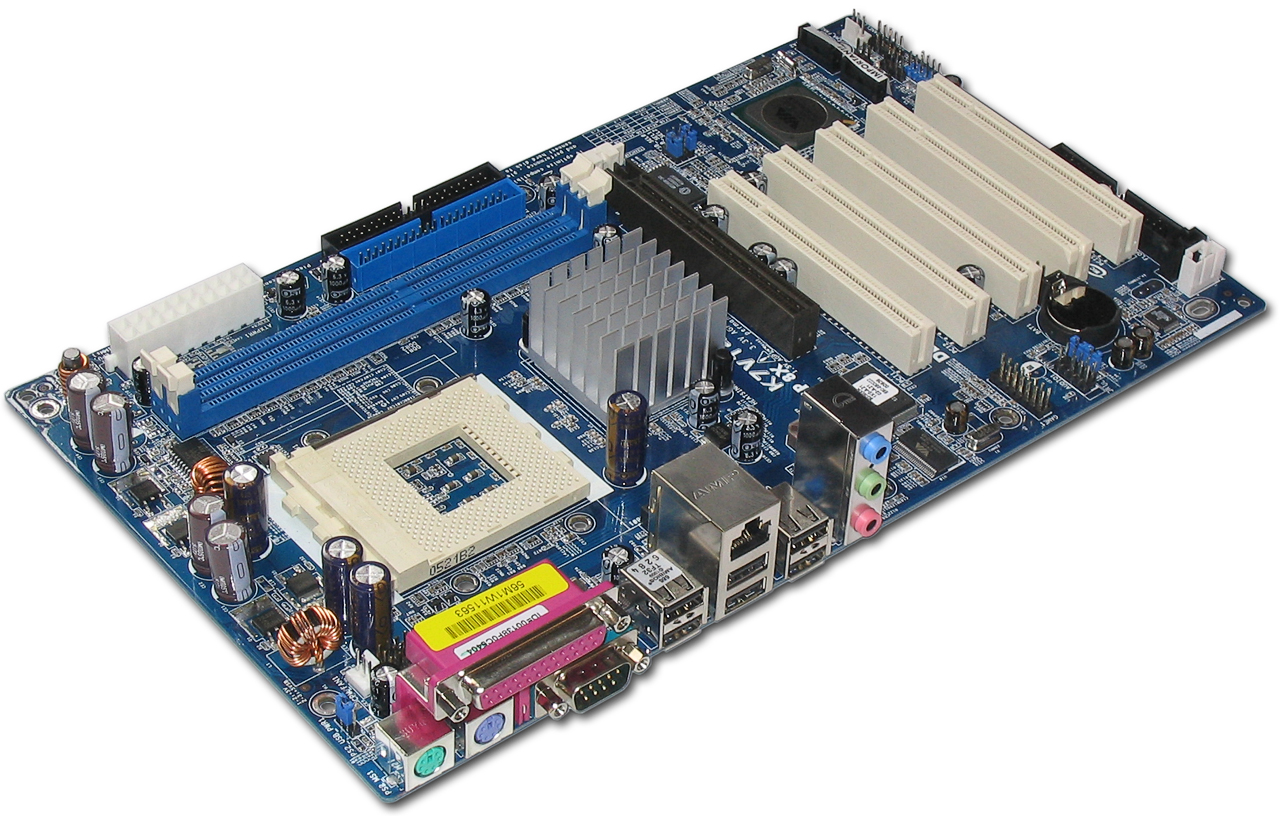
\includegraphics[width=4cm]{images/cartemere}};
	\node (image5) at (0,12) {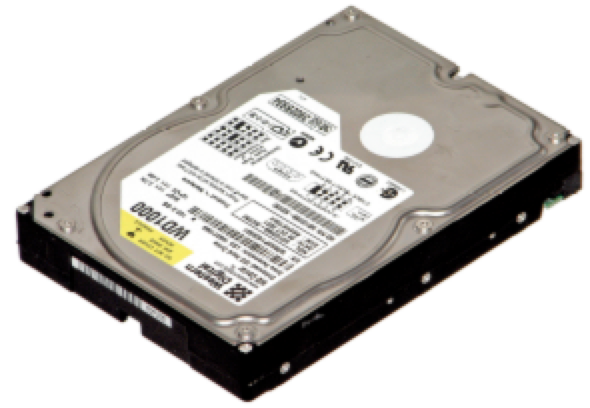
\includegraphics[width=4cm]{images/disquedur}};
	\node (image6) at (0,15) {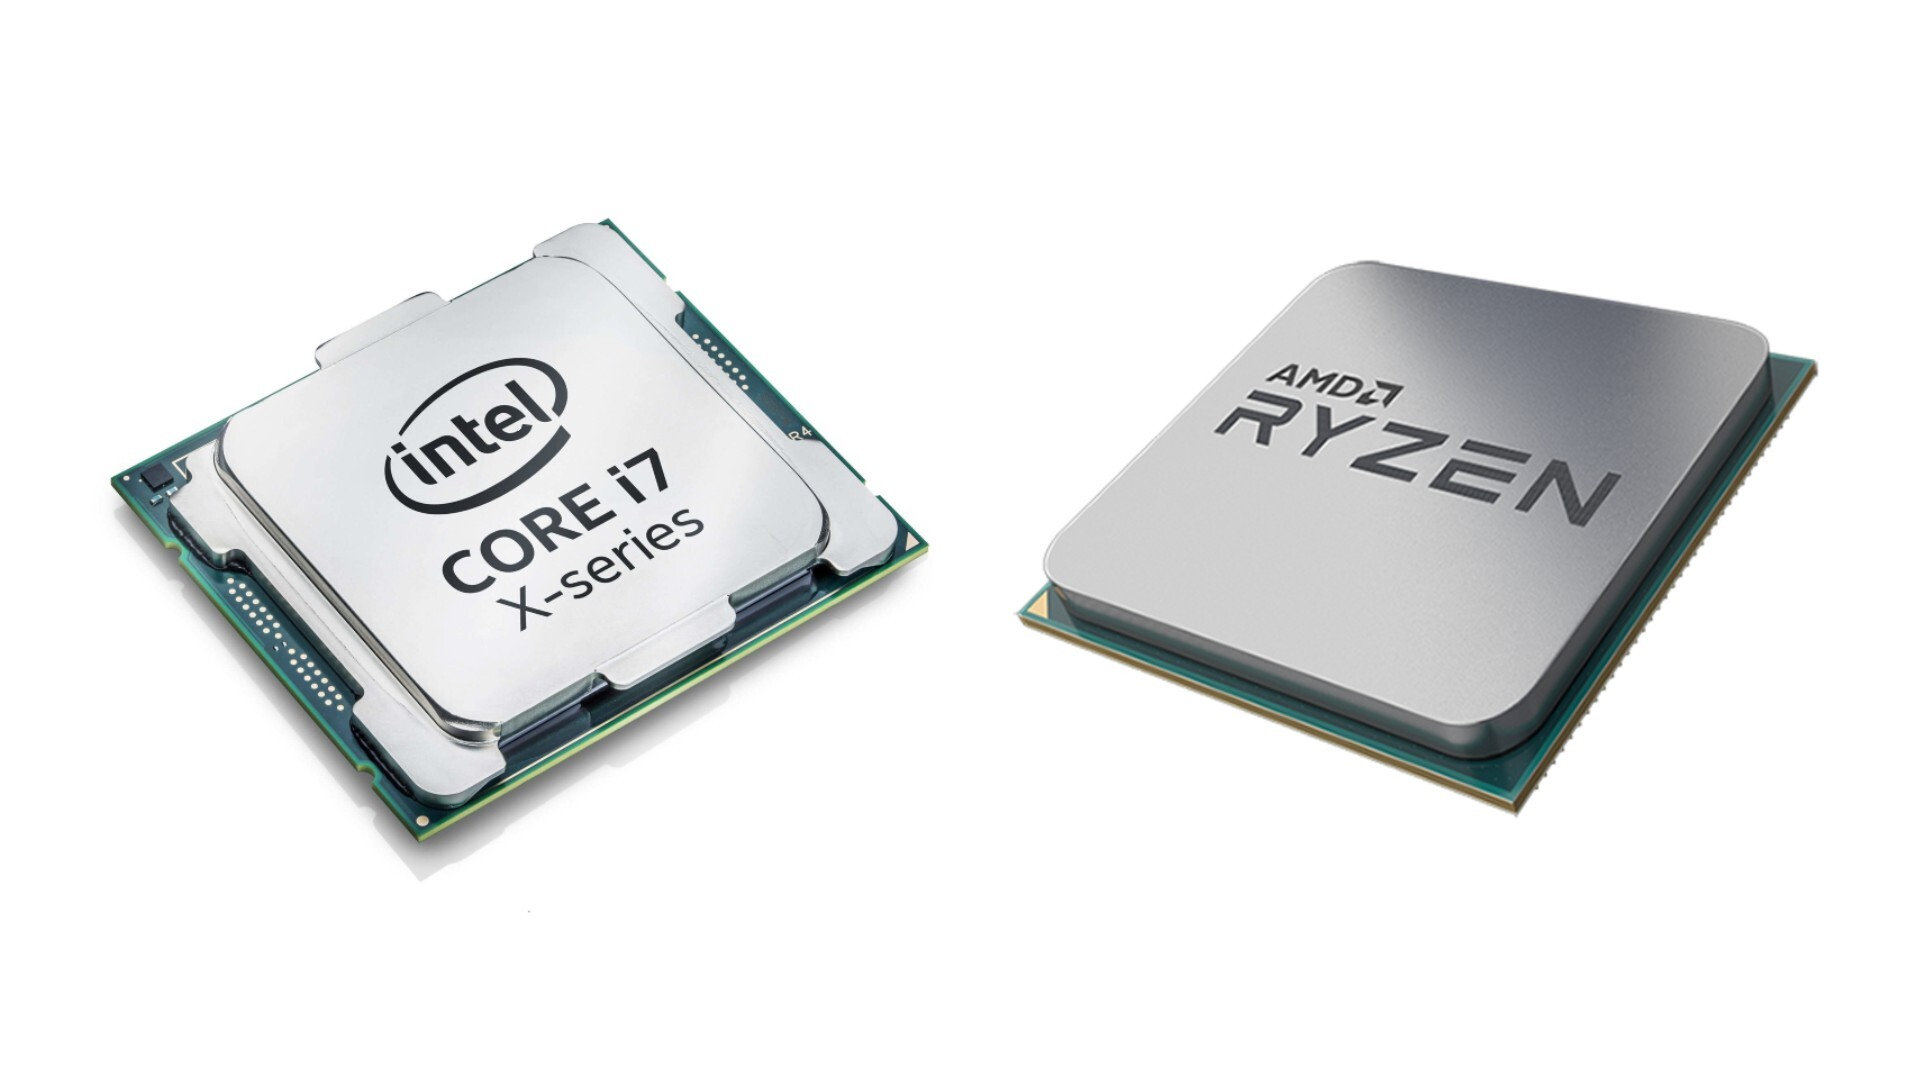
\includegraphics[width=4cm]{images/processeur}};
	
\filldraw[fill=black] (4,0) rectangle +(0.3,0.3);	
\filldraw[fill=black] (4,3) rectangle +(0.3,0.3);	
\filldraw[fill=black] (4,6) rectangle +(0.3,0.3);	
\filldraw[fill=black] (4,9) rectangle +(0.3,0.3);	
\filldraw[fill=black] (4,12) rectangle +(0.3,0.3);	
\filldraw[fill=black] (4,15) rectangle +(0.3,0.3);	
	
\begin{scope}[shift={(3,0)}]	
	\filldraw[fill=black] (4,0) rectangle +(0.3,0.3);	
	\filldraw[fill=black] (4,3) rectangle +(0.3,0.3);	
	\filldraw[fill=black] (4,6) rectangle +(0.3,0.3);	
	\filldraw[fill=black] (4,9) rectangle +(0.3,0.3);	
	\filldraw[fill=black] (4,12) rectangle +(0.3,0.3);	
	\filldraw[fill=black] (4,15) rectangle +(0.3,0.3);	
\end{scope}

\draw (8,9.2) node[right] {L'alimentation};
\draw (8,6.2) node[right] {Carte graphique};
\draw (8,3.2) node[right] {Le disque dur};
\draw (8,0.2) node[right] {Processeur};
\draw (8,12.2) node[right] {Carte mère};
\draw (8,15.2) node[right] {Mémoire vive (RAM)};
	
\end{tikzpicture}
\end{exercice}



\begin{exercice}
Réponds aux questions suivantes :
\begin{enumerate}
\item Je suis le circuit imprimé principal où tous les composants sont reliés. 

\vskip.5cm

Je suis :

\vskip.5cm

\item  Je gère tous les calculs pour permettre à l’ordinateur de fonctionner. \vskip.5cm

Je suis :

\vskip.5cm
\item  Je suis connecté à l’ordinateur et j’affiche tout ce qu’il m’envoie comme du texte, des dessins, des photos, des films, etc.
\vskip.5cm

Je suis :

\vskip.5cm
\item Je m’appelle mémoire permanente et je conserve toutes les données même si l’ordinateur est éteint.
\vskip.5cm

Je suis :

\vskip.5cm
\item Sans moi, on ne peut pas taper du texte. 
\vskip.5cm

Je suis :

\vskip.5cm
\item Je suis une mémoire plus rapide que la mémoire permanente et je ne conserve pas les données si l’ordinateur est éteint.
\vskip.5cm

Je suis :

\vskip.5cm

\end{enumerate}

\end{exercice}



\begin{exercice}
{\bf Complète le schéma.}

Le schéma suivant représente les différents périphériques externes d’un ordinateur. Dessine le sens des flèches pour indiquer si le périphérique est en entrée ou en sortie.

{\it Par exemple : le clavier est un périphérique d’entrée, il y a donc une flèche qui part du clavier à l’unité centrale.}

\begin{figure}[h!]
\centering
	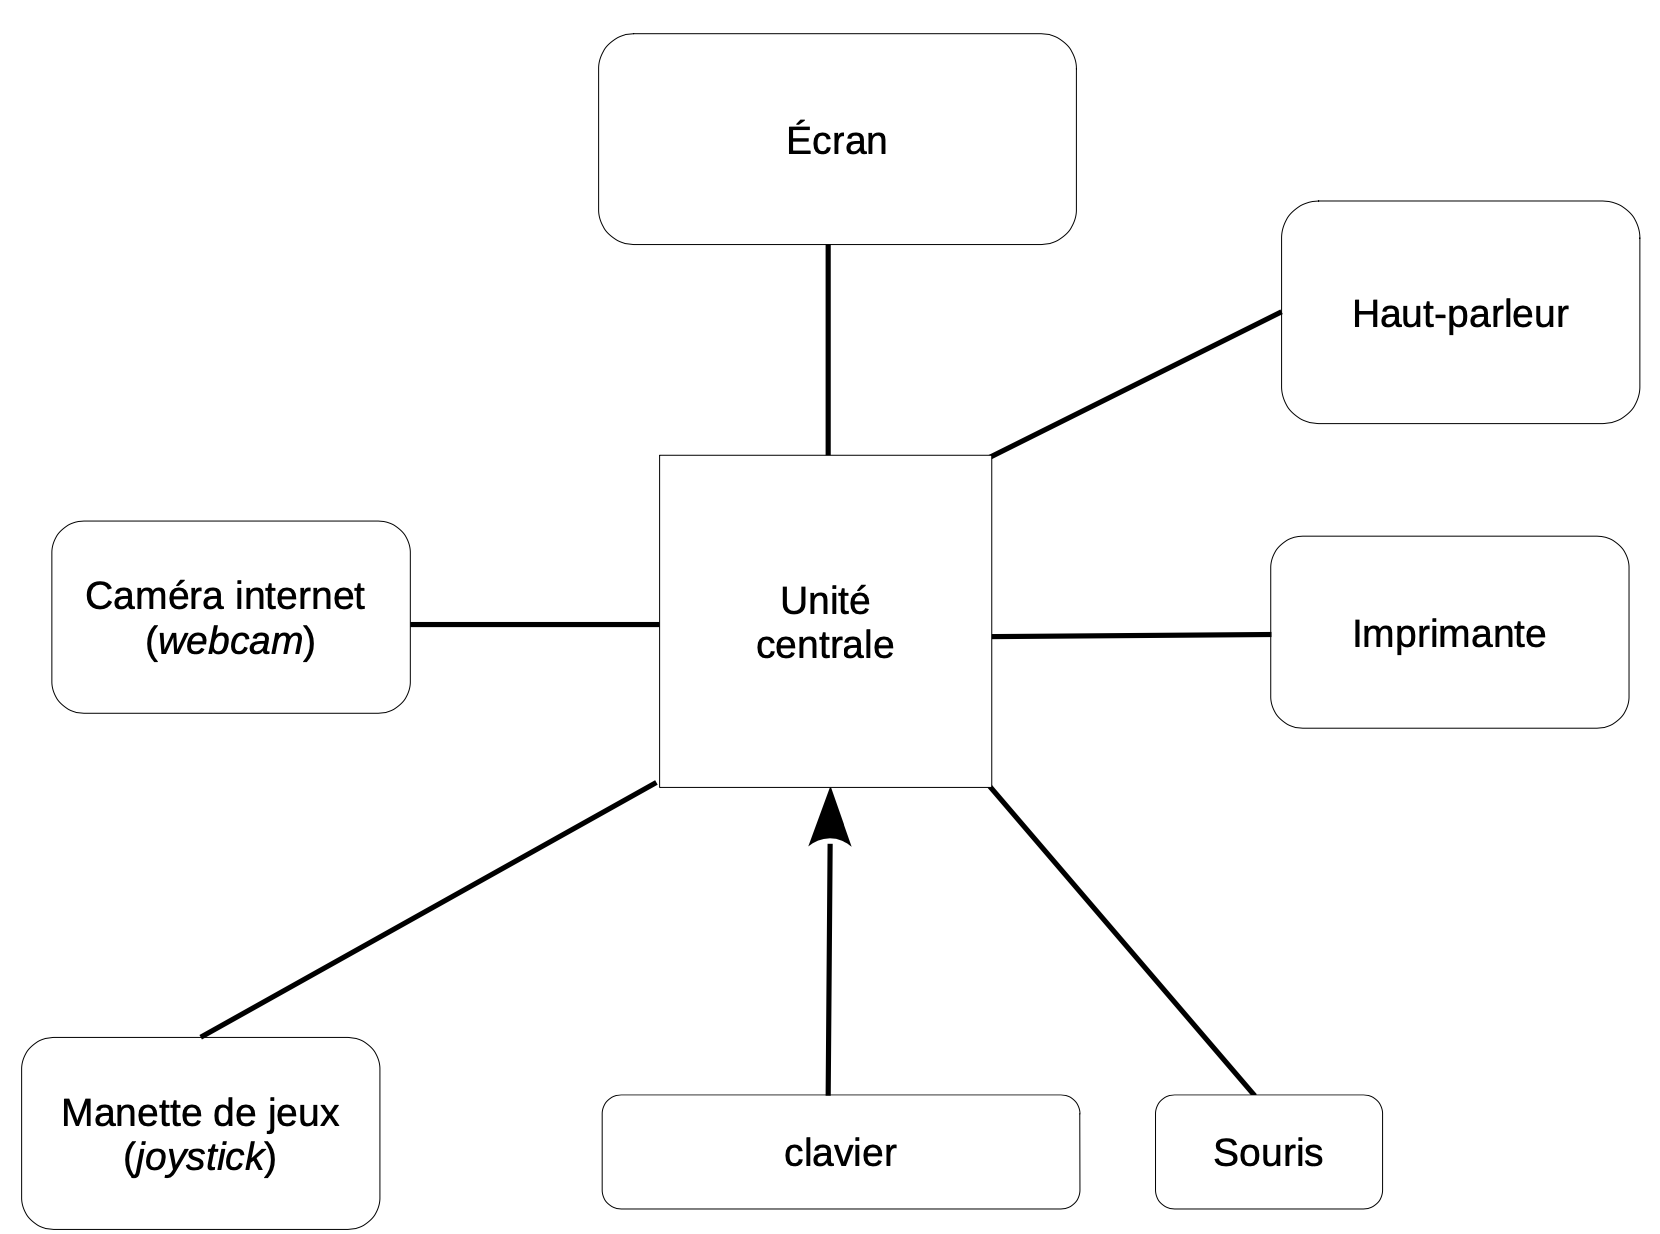
\includegraphics[width=14cm]{images/ordinateur_ex_3}
\end{figure}
\end{exercice}


\end{document}